\documentclass[10pt]{article}
\usepackage{common}
\usepackage{dirtree}
\usepackage[section]{placeins}
\usepackage{float}
\usepackage[colorlinks=true, urlcolor=blue]{hyperref}
\pagestyle{plain}
\title{CS182 Final Project}
\author{Nikhil Suri and Soumil Singh}
\date{December 18, 2018}
\begin{document}
\maketitle{}

\begin{center}
    \href{https://github.com/RealDealNikhil/tetris-agent}{Click Here To Access Github Repository}
\end{center}

\section{Introduction}
The initial goal in undertaking this project was to investigate the possible application of Q-learning for the game of Tetris. More specifically, we wanted to apply Q-learning techniques to create an agent which could learn how to optimally play the game i.e. optimally 'clear lines' and survive for as long as possible. Our goal was to compare the effectiveness of exact Q-learning techniques (model-free learning) against approximate Q-learning techniques (model-based learning) for different specifications of the game, that is, for different sizes of the game board and under different models of rewards. We hypothesised that in general an approximate Q-learning learning agent would perform better than an exact Q-learning agent predicated on the reasoning that our defined state-space would be very large, and thus our exact Q-learning agent wouldn't sufficiently explore the state-space in time to conduct its learning. To substantiate this comparison, we also had the goal of comparing the effectiveness of the two different agents for different boards (i.e. differently sized state-spaces), different learning parameters (i.e. different learning rates $\alpha$ and different random-action selection rates for epsilon greedy approach $\epsilon$), and different heuristics/features for the approximate Q-learning agent. After conducting analysis on these manifold aspects, we have the goal of drawing conclusions regarding what an optimal Q-learning agent for this game might look like.

The Q-learning algorithms we applied, detailed in the Approach section, were fundamentally the same algorithms we learnt in class. However, we created our own representation for states and actions for the tetris game. Furthermore, we defined our own features for approximate Q-learning, and implemented our own methods for testing both agents. We tested against two baseline agents: one was a random-action agent, which picks any legal action with equal probability. The other was a greedy agent, which chooses actions based on a naive application of two heuristics. We utilised an existing pygame version of tetris, with a pre-defined implementation of the tetris board, pieces, and user-interaction (key-board presses) functionality; we built upon this framework to implement our Q-learning agents by defining our own representation for states, legal actions, rewards, storage of Q-values, any by implementing our two main Q-learning algorithms.

\section{Scope}

\subsection{Background and Related Work}
To apply these Q-learning approaches to tetris, we used an existing pygame representation of the tetris game \cite{WEBSITE:1}; thus, we had access to code which defined the board, pieces, keyboard-moves, and all visual representation. We then created our own representations for states and actions (the definitions of which can be found in the section titled 'problem specification') for which our agents would learn with. We then applied the feature based and exact Q-learning algorithms we learnt during this course. We utilised a similar structure to that in the Reinforcement Learning problem set to define the 'RLAgent' class \cite{CODE:1}. We also utilised an iterative depth-first search to define one of the heuristics that we used for approximate learning. This application of depth-first search was also adapted from our implementation in one of the problem sets \cite{CODE:2}.

\subsection{Problem Specification}
The specific problem that we are investigating is how well reinforcement learning, through exact and approximate q learning, can be applied to the game of Tetris. To apply reinforcement learning to Tetris, we must have a formal definition of the game, the state space, and the action set of Tetris.

\subsubsection{Game}
The game of Tetris is played on a board of width $w$ and height $h$. This board initially starts off empty. During each turn, the player is given a piece to place on the board that begins falling from the top of the board. The player can rotate and move this falling piece from side to side. As the player places more pieces on the board, the stack of pieces rises higher and higher. If the stack of pieces rises too high and the player cannot place a piece anywhere on the board, then the game is over. The player attempts to keep the stack of pieces on the board low by clearing lines: every time the player fills an entire row of blocks, that line is cleared from the game board and all blocks above that row shift down. The player also scores points by clearing lines. The goal of the game is score as many points as possible. This is done by clearing lines, and thus by continuing to play for as long as possible.

\bigskip

In addition to knowing the entire board configuration and falling piece, the player is told what the next piece will be (pieces are assumed to spawn randomly). The player also has the option to place a piece in "reserve" and save it for later. The idea behind this is that by putting a piece in reserve, the player can plan to use the piece to clear lines later or temporarily escape from a situation where there are no locations that the player deems to be "good" to place the piece.

\bigskip

For our project, we have slightly simplified Tetris. In real Tetris, part of the challenge of placing pieces on the board (in addition to choosing the best rotation and column to drop the piece in) is actually getting the piece to the column in which you want to drop it. Pieces spawn in the center at the top of the board and fall at a certain rate. The rate at which pieces fall is determined by how many lines the player has cleared. Once a falling piece touches the stack of pieces already on the board, it becomes stuck, and the player can no longer move it. In some versions of Tetris, there is additional complexity where, for a short time after the piece touches the stack, the player can continue to move it from side to side and rotate it. Currently, we do not support these features in our implementation of the game. We also currently do not allow the agent to hold a piece in reserve. In our implementation, the agent is simply given a piece which it can place anywhere atop the current stack of pieces on the board and is allowed unlimited compute time.

\subsubsection{State Space}
Tetris has a huge state space. Each square on the board can either have a block in it or not. If we let $w$ be the width of the board and $h$ be the height of the board, then the number of possible board configurations is $$2^{w\cdot h}$$
Now, an important observation is that we will never reach a board configuration where there are rows which are full of blocks (these rows will be cleared, according to the rules of Tetris). Therefore, this is a counting problem: the number of board configurations which have a single row of full blocks is
$$\binom{h}{1}2^{w\cdot(h-1)}$$
The number of configurations which have 2 rows of full blocks is
$$\binom{h}{2}2^{w\cdot(h-2)}$$
and so on. Therefore, in reality the number of possible states is
$$2^{wh} - \sum_{k=1}^{h}\binom{h}{k}2^{w\cdot(h-k)}$$
However, we note that this reduction is really of no help. A typical board in Tetris is 10x20 squares, which by our calculation has
$$2^{200} - \sum_{k=1}^{20}\binom{20}{k}2^{10\cdot(20-k)}=1575259648227583387903265739476252776198605528180667457712127$$
possible states. Even on a smaller board with dimensions 5x8, we will still have
$$2^{40} - \sum_{k=1}^{8}\binom{8}{k}2^{5\cdot(8-k)}=792614637311$$
possible states. Clearly, training an exact Q Learning agent, which stores entire board configurations as states, is not feasible for Tetris. We must also consider that a state does not consist solely of a board configuration; in Tetris we are also know what the falling piece and next piece are. Since there are 7 pieces in Tetris, our state space is already larger by a factor of 49. Therefore, an exact Q Learning agent requires a much more concise way of representing states. Here, we introduce the concept of the "top line" of a board. The top line of a board is the $w$ (where $w$ is the width of the board) free spaces (not occupied by blocks) which are at the top of each column of the board. This greatly reduces our state space. To count the number of possible top line configurations that there are in a board of width $w$ and height $h$, let us first consider the number of ways to place blocks in a single column. In a single column, there are $h$ ways to arrange blocks ($h$ locations to place a block). In 2 columns, there are $h^2$ ways to arrange blocks. We need to correct for counting complete rows. The number of permutations where all of the blocks are in the same row is $h$. Therefore, the total number of top line configurations that we will have is
$$h^w - h$$
For a typical board of size 10x20 the number of top line configurations will be
$$20^{10} - 20 = 10239999999980$$
This is still quite large. However, for a smaller board of size 5x8 the number of top line configurations will be
$$8^5 - 8 = 32760$$
Now this is a feasible state space size! We can make this even smaller if we consider the effect of "normalization". By normalization, we mean that we can "normalize" a (row, col) top line of $((2,0),(2,1),(1,2),(1,3),(2,4))$ to $((1,0),(1,1),(0,2),(0,3),(1,4))$. The key observation is that we would want the same action that occurs in the latter top line to occur in former top line, because the agent should be selecting the optimal action in both cases. Normalization therefore has the effect of always reducing a top line to one which has at least one column which is empty. To calculate the effect which normalization has, let us consider the case where there is one empty column on the board. The number top lines we can have is
$$h^{w-1}\binom{w}{1}$$
If there are two empty columns, the number of top lines we can have is
$$h^{w-2}\binom{w}{2}$$
Therefore, with normalization, the total number of top lines we can have for a board with width $w$ and height $h$ is
$$\sum_{k=1}^{w-1}h^{w-k}\binom{w}{k}$$
On a typical board of size 10x20 the number of normalized top lines will be
$$\sum_{k=1}^{9} 20^{10-k}\binom{10}{k} = 6439880978200$$
On the smaller board of size 5x8 the number of normalized top lines will be
$$\sum_{k=1}^{4} 8^{5-k}\binom{5}{k} = 26280$$
Adding in the falling piece and next piece, we see that on a board of size 5x8 the size of the state space will be
$$(49)(26280) = 1287720$$
Although large, this state space is still manageable for exact learning. For approximate learning, we do not need to worry about reducing the state space so much. In approximate learning, we do not need to store a table of (state, action) pairs. We determine the value of a state by using heuristics which are calculated based on the current configuration of the entire board, the falling piece, and the next piece. Therefore, our states for approximate Q-learning are simply the entire board configuration, the falling piece, and the next piece.

\subsubsection{Action Set}
Given a state, we have defined the set of legal actions for that state as (rotation, column) pairs. Here, rotation is a number that represents which rotation a falling piece is in. Column is a number that represents which column we are dropping the piece now, with respect to the top left corner of that piece in its rotation. Once an action is chosen, we will set the rotation of the falling piece, move it over to the column which we want to drop it down, and drop it as far down as it can go in that column. The maximum number of rotations for any piece is 4. In a board of width $b$, the maximum number of columns which we can drop a piece down is  $b$. Therefore, there are at most $4b$ actions for every piece. Since there are 7 different pieces in Tetris, the number of different actions there are is at most $28b$. We use the same action set for approximate learning as we do for exact learning.

\section{Approach}

\subsection{Game Implementation}
The implementation of the game itself is adapted from "Tetronimo" (a Tetris clone) by Al Sweigart. Many of the functions used to draw objects on the screen and manipulate the game board (such as clearing lines and dropping pieces) were written by him\cite{WEBSITE:1}. We adapted the game to be Object-Oriented: each piece object is generated by an object called the "piece generator". The board object then has functions to manipulate the board itself. The game board itself is stored as a column-wise list of lists. For our Exact Learning agent, we store states as tuples of the board's top line, the shape of the falling piece, and the shape of the next piece. For our Approximate Learning agent, we store states as tuples of the current board, the shape of the falling piece, and the shape of the next piece. For both agents, actions are stored as tuples of (rotation, column) pairs.

\subsection{Algorithms}
The main algorithms that we used were the Exact Q Learning and Approximate Q Learning algorithms \cite{CODE:3}. As defined in the lecture notes, the Exact Q Learning algorithm stores a lookup table of (state, action) pairs with their associated Q-values. To update Q-values in the case of exact Q-learning, we use the following algorithm where $s$ and $a$ are the previous state and action, $s'$ is the new state, $r$ is the observed reward, $\gamma$ is the discount factor, and $\alpha$ is the learning rate:
\begin{algorithm}[H]
  \begin{algorithmic}
    \Procedure{updateQValues}{$s, a, s', r$}
        \State{$sample \gets r + \gamma\max_{a'}Q(s', a')$}
        \State{$Q(s,a) \gets Q(s,a)(1 - \alpha) + \alpha\cdot sample $}
    \EndProcedure{}
  \end{algorithmic}
  \caption{Exact Q Learning Q-value Update}
\end{algorithm}
As defined in the lecture notes, the approximate Q Learning algorithm stores a table of weights associated with pre-defined features. These features are obtained by evaluating certain heuristics on a (state, action) pair. The Q-value of a state thus becomes the dot product of the feature and weight vectors:
$$Q(s,a) = w_1f_1(s,a) + w_2f_2(s,a) + \ldots + w_nf_n(s,a)$$
To update values for the weights, we use the following algorithm where where $s$ and $a$ are the previous state and action, $s'$ is the new state, $r$ is the observed reward, $\gamma$ is the discount factor, and $\alpha$ is the learning rate:
\begin{algorithm}[H]
  \begin{algorithmic}
    \Procedure{updateWeights}{$s, a, s', r$}
        \State{$difference \gets \alpha(r + \gamma\max_{a'}Q(s', a') - Q(s,a))$}
        \For{i = 1:n}
            \State{$w_i \gets w_i + f_i(s,a)\cdot difference $}
        \EndFor{}
    \EndProcedure{}
  \end{algorithmic}
  \caption{Approximate Q Learning Weights Update}
\end{algorithm}
For our implementation, we adopted some of the code we used for problem set 3 on reinforcement learning in pacman. To store our Q-value and weight lookup tables, we used the \texttt{Counter} object defined in \texttt{util.py}.

\bigskip

We also utilized $\epsilon$-greedy action selection and a depth-first search for one of the heuristics that we defined for our approximate learning agent.

\subsection{Rewards}
We used 3 different reward models to test our agents. Below is a description of each. We will discuss the results and effectiveness of each in the results section:
\begin{enumerate}
    \item The first rewards model we defined used a "living penalty" of -1 for any move that did not result in a line clear. Line clears were scaled up by 1000 so that clearing a single line would result in a reward of 1000, clearing 2 lines would result in a reward of 2000, etc. There was no "losing penalty" enacted when the agent lost the game. The idea behind this model was that it might incentivize the agent to make line clears as fast as possible.
    \item The second rewards model we defined has no penalty for moves that do not result in line clears. There is only a penalty for losing of -0.5. Line clears are scaled down by 1000. Therefore, clearing a line results in a reward of 0.001, clearing 2 lines results in a reward of 0.002, etc. The idea behind this model was that it could incentivize the agent to stay alive for as long as possible.
    \item The third rewards model we defined combines the living penalty for making moves that do not result in line clears with the penalty for losing and the scaled down penalty for clearing lines. We also kept the losing penalty of -0.5 from model 2. Given a board width of $b$, we set the living penalty to be $-0.001/b$. The idea behind this is that the agent should be clearing lines about as often as they get enough pieces to fill up the width of the board.
\end{enumerate}

\subsection{Heuristics}
We defined and tested several heuristics for approximate learning. In our feature extractor, we calculated features given a state-action pair. To do this, we made a copy of the current board-representation (so that by performing the given 'action', the actual board was not edited) and performed the action on this copy. Then, we calculated heuristics on this board-copy to assess what our 'features' would be if we performed a particular action on a particular current board representation. Thus, given a (state, action) pair, our heuristics  were calculated as follows:
\begin{enumerate}
    \item \textbf{Highest Point:}
    This refers to the highest point on the current 'stack' on the board, where the stack refers to the amalgamation of pieces below the empty space at the top of the board. We anticipated that our approximate agent would learn negative weights for this feature, because a larger 'highest point' would, by proxy, imply a higher 'piece stack', which would mean our agent is closer to breaching the top of the board and dying.
    \item \textbf{Aggregate Height:}
    This is the sum of all the highest points of each column of the current stack of blocks that are on the board. This is another feature which we would expect our agent to learn a negative weight for, because a higher aggregate height means that our agent is closer to the top of the board and losing.
    \item \textbf{Holes:}
    The number of 'Holes' refers to the number of blank-spaces below the top line of our 'piece stack'. They define the empty spaces that are currently inaccessible to our agent, i.e. there exists a filled space at some height above the height of the 'hole'. We anticipated that our approximate Q-learning agent would learn negative weights for this feature, because a greater number of holes implies our 'piece-stack' is not optimally compressed; this means that it is 1) more likely that our 'piece-stack' is taller, and 2) future line-clears could be more difficult for our agent. In both cases, it would seem our agent should seek to minimize this feature.
    \item \textbf{Squared Hole Size:}
    The idea behind squared hole size was to not just naively count the number of 1x1 empty spaces on the board. Squared hole size redefines a "hole" on the board as any group of empty spaces that are adjacent to each other on the board and below the top line of the board (and thus inaccessible). To find the size of each "hole" (using this new definition of hole), we keep a set of all of the 1x1 holes on our board that are below the top line. Then, we run a DFS on this set of 1x1 holes, counting the size of each hole that consists of connected 1x1 holes. We catch the case where our DFS ventures above the top line (and thus into empty space above the top line) in some other column. We also expected our agent to learn a negative weight for this feature because a higher squared hole size means that it is harder to clear lines on the board.
    \item \textbf{Lines Cleared:}
    This feature refers to the number of complete Lines that would be cleared after taking the specified action, where a 'complete line' refers to a row on the Tetris board in which every space is filled by a piece. We expect our approximate agent to learn a positive weight for this feature, since maximizing this feature would seem to maximize agent rewards.
    \item \textbf{Height Difference:}
    This feature measures the "bumpiness" of the board. This is defined as the average difference between the heights of all adjacent columns on the board. We expected our agent to learn a negative weight for this feature because a very bumpy board would make it hard to neatly fill rows and clear lines on the board.
    \item \textbf{Bias:}
    The idea behind this feature is that often, when learning approximations, there is a constant factor in addition to any features that we define. For example, in linear regression, we are trying to learn the equation $y = \theta_1x + \theta_2$, where $\theta_1$ and $\theta_2$ are our weights and $\theta_2$ is a constant that must be learned. Therefore, this bias feature is always set to 1 (this bias feature was also included in the reinforcement learning problem set \cite{CODE:1}).
\end{enumerate}
After calculating the value for each feature on a board of width $w$ and height $h$, we scale all of our features down by $w\cdot h$. Since the "squared hole size" feature tends to be quite large, we scale that feature down by an additional factor of $w \cdot h$.

\section{Experiments}

\subsection{Methodology}
Testing our agents took up a significant portion of our time to complete this project. The challenge of testing our exact learning agents was that there are so many Q-values, so learning an effective policy could take hundreds of thousands of iterations. The challenge of testing our approximate learning agents was that there were many features to compare against each other, and sometimes our agents learned weights for features so well that they continued to play for a very long time during testing! Therefore, to obtain more visibility through our training and testing runs, we trained and tested our agents in sets of games and recorded average scores over training and testing episodes. For example, we often trained our exact learning agents on sets of 50000 games, checked and recorded our results, and then loaded in the learned q-values and tested for another 50000 games. We did the same for our approximate agents, though they needed many fewer training games. To export and import q-values and weights across training and testing runs, we used the python library \href{https://docs.python.org/2/library/pickle.html#module-cPickle}{cPickle}.

\bigskip

We wanted to compare the performance of our rewards models and agents (random, exact, and approximate) against each other. However, before we could accurately compare results across models, we had to gain a better understanding of what kinds of learning parameters and board sizes would work best for our agents. Therefore, much of our testing also involved varying board sizes and learning parameters. When comparing results across different models and agents then, we decided to standardize to a 5x8 board, with $\alpha=0.01$, $\epsilon=0.2$ and $\gamma=1$. We also defined a couple of naive agents to use for baseline testing. The naive agents that we use are a random agent and a greedy agent. The random agent picks a random action to take in every state. The greedy agent chooses the action that will maximize the number of line clears in a certain state. If no actions result in any line clears, then the greedy agent will choose the action that minimizes the number of holes.

\subsection{Results}

\subsubsection{Baselines}
We tested our baseline agents on 5x8 and 10x20 boards. For the 5x8 boards, we took average line clears over 10K games (similar to how we tested our exact agents). For the 10x20 boards, we took average line clears over 900 games (similar to how we trained/tested our approximate agents). Below are the results for each:
\begin{table}[H]
  \centering
  \begin{tabular}{lll}
    \toprule
    Agent & Board & Score \\
    \midrule
    Random & 5x8 & 0.73\\
    Greedy & 5x8 & 9.74\\
    Random & 10x20 & 0.11\\
    Greedy & 10x20 & 13.6\\
    \bottomrule
  \end{tabular}
  \caption{Average Line Clears on 5x8 and 10x20 boards.}
\end{table}
Some intuition as to why the Random agent performs worse on the 10x20 board than on the 5x8 board is that it is likely much easier to randomly get line clears on the 5x8 board because it has a smaller width. We suspect that the greedy agent does not perform much better on the 10x20 board because of the larger width, and because it is not taking into account and weighting other features such as the height, bumpiness, or size of the holes.

\subsubsection{Exact vs. Approximate Learning}
Our approximate learning agent completely outperforms our exact learning agent. Typically our exact learning agents took around 500000 training games to get to a point where they could clear just 7 lines per game on average on a 5x8 board. Our approximate agents were able to clear, on average, 20 lines per game on a 5x8 board after only 500 training games. The graph below shows the comparison between the performance of approximate and exact learning on a 5x8 board over 3000 training games:\\
\begin{center}
    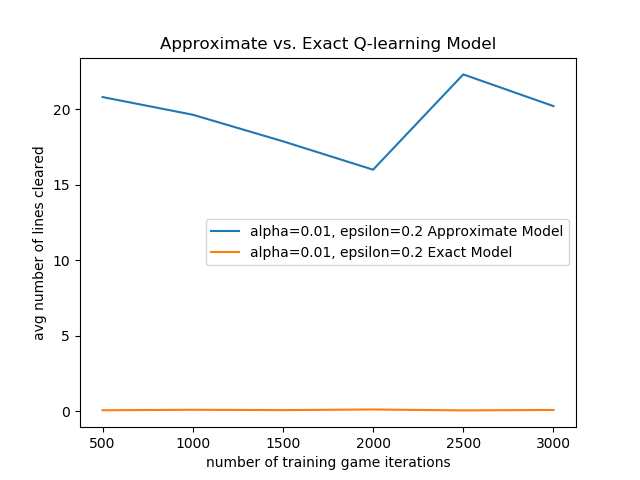
\includegraphics[scale=0.50]{exactvsapprox.png}
\end{center}

\subsubsection{Heuristic Comparisons}
We defined 4 sets of feature combinations to train our approximate agents on for comparison:
\begin{enumerate}
    \item number of holes, highest point, bias, height difference.
    \item squared hole size, highest point, bias, height difference.
    \item number of holes, aggregate height, bias, height difference.
    \item squared hole size, aggregate height, bias, height difference.
\end{enumerate}
We decided on these sets of feature combinations because we felt that it would be redundant to include both the number of holes and the squared hole size, or the highest point and the aggregate height, features in the same set. We kept the average height difference feature in all of the feature sets because there was no other feature that we felt would be redundant if included with this feature. Since the bias feature represents a constant factor in our approximation, we kept that in all of our feature sets. After some initial testing, we chose to not include the "number of lines cleared" feature, because this feature is already captured in the agent's reward. Below is a graph of our results for each of the feature sets, over 900 total training games with average results taken every 300 games over 20 testing games:
\begin{center}
    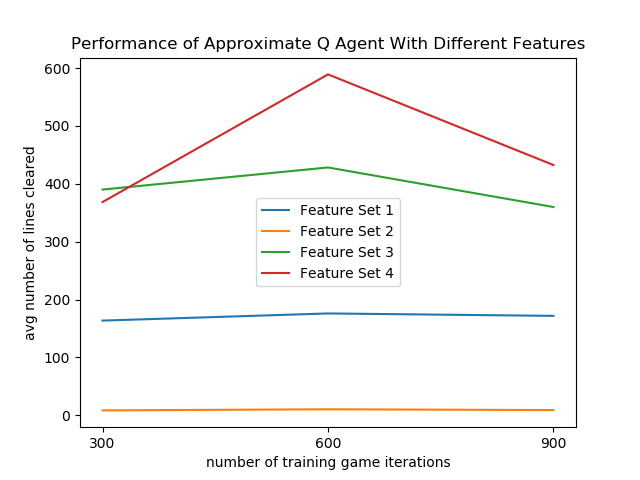
\includegraphics[scale=0.50]{heuristics.png}
\end{center}

In general, the feature 'aggregate height' seemed to produce better results than the 'highest point' feature, as evidenced by the superior performance of the agent when trained with feature sets 3 and 4. Intuitively, Most interestingly, feature set 2 produced the worst results, but feature set 4 produced the best, where the only difference between feature sets 2 and 4 is that the 'height' feature is highest point in set 2, and aggregate height in set 4. In other words, in the case we used the squared hole size heurtistic, we get the both the best and worst agent performances depending on which feature for 'height' we use.

\subsubsection{Learning Parameters and Board Sizes}
We mainly experimented with varying the learning parameters for $\alpha$ and $\epsilon$, while keeping $\gamma$ constant at a value of 1. The intuition behind this was that we wanted our agents to always be planning for the future as much as possible, since in tetris line clears do not happen after every single move. Training and testing agents took a very long time. Ideally, given more time, we would also like to experiment with varying our value of $\gamma$. We found that low values of $\alpha$ generally gave the best results. We think this may be the case because, again, line clears do not happen very often. Therefore, it is important to not "overwrite" old information at too fast a rate. We also experimented with different board sizes for our agents. We found that the exact learning agent performed worse on wider boards and better on taller boards. We think this may be the case because wider boards make it much harder to clear lines, while taller board allow the agent to stay alive for longer and thus clear more lines. Below are some graphs detailing our results:
\begin{figure}[H]
  \centering
  \begin{minipage}[b]{0.4\textwidth}
    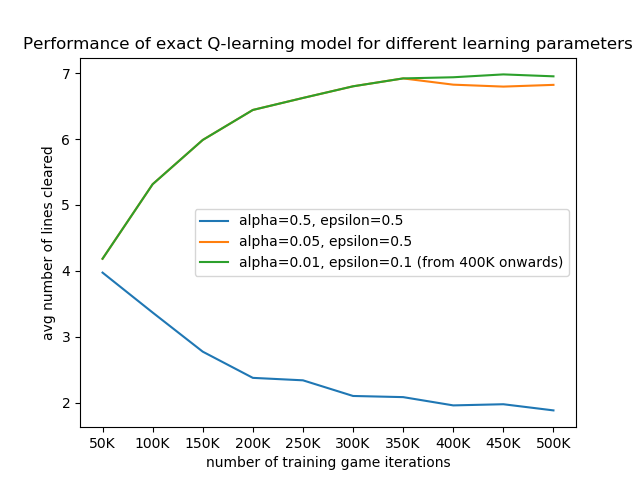
\includegraphics[scale=0.50]{exactQparameters.png}
  \end{minipage}
  \hfill
  \begin{minipage}[b]{0.4\textwidth}
    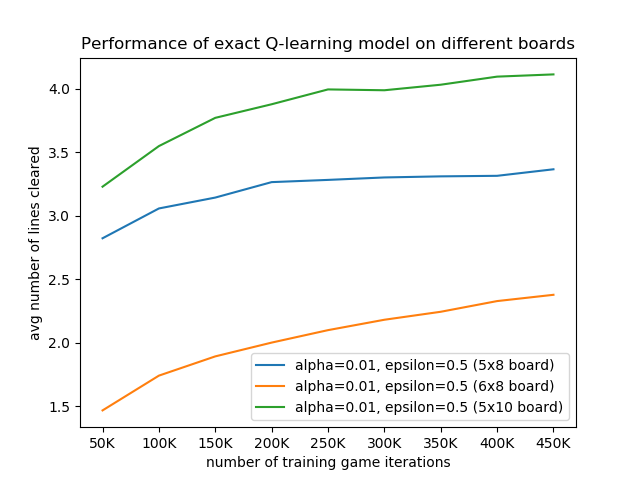
\includegraphics[scale=0.50]{boardsize.png}
  \end{minipage}
\end{figure}
Based on these results, we decided to standardize our testing for comparing agents and rewards models against each other to use a 5x8 board with $\alpha=0.01$, $\epsilon=0.2$, and $\gamma=1$.

\subsubsection{Rewards Model Comparisons}
Testing the reward models yielded results that were very interesting. Our exact learning agent performed the best under rewards model 1 and the worst under model 3. Meanwhile our approximate agent performed the best under model 2. Our approximate agent performed terribly under model 1 - its weights wildly diverged and it was barely able to clear even a single line on average per game. We therefore did not feel the need to include the results of our approximate agent under model 1 because they were essentially meaningless. Below are some graphs which go into further detail (our exact agents were trained on 5x8 boards, while our approximate agents were trained over 300 and tested over 20 games on 10x20 boards):
\begin{figure}[H]
  \centering
  \begin{minipage}[b]{0.4\textwidth}
    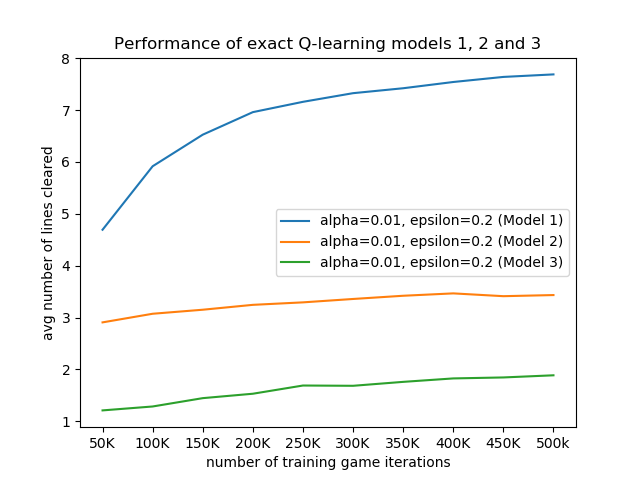
\includegraphics[scale=0.50]{exactmodels123.png}
  \end{minipage}
  \hfill
  \begin{minipage}[b]{0.4\textwidth}
    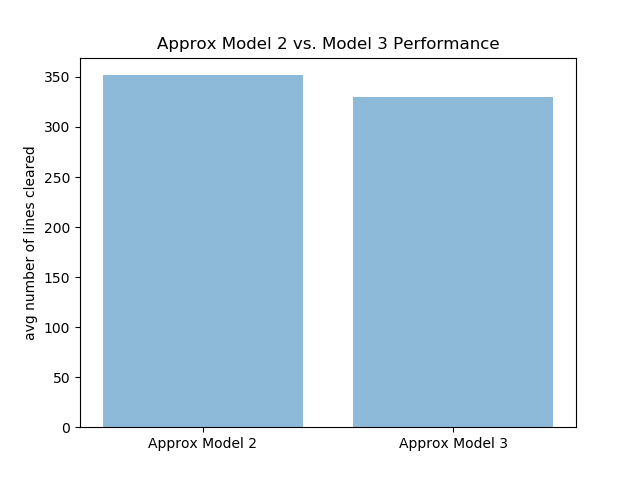
\includegraphics[scale=0.50]{approxmodel23.png}
  \end{minipage}
\end{figure}

\section{Discussion}
In this section we will discuss the intuition behind some of the results that we found, critically evaluate the ways in which we tested our agents, and consider ways in which, given more time, we could improve the testing of our agents and extend the project so that it becomes more similar to real Tetris.

\bigskip

One of the fundamental questions we posed in this study asked whether the exact or approximate Q-learning models would perform better in this game. We hypothesized that because of the large number of states in tetris, even for a board of size 5x8, that exact Q-learning would require very large amounts of training iterations to explore the possible states for which to learn Q-values for. We therefore argued that this would mean our approximate Q-learning model(s) would significantly outperform our exact models; this hypothesis proved to be true. With reference to our graph titled 'Approximate vs. Exact Q-learning Model', we see that after 3000 training game iterations the approximate Q-learning agent, on the 5x8 board, clears approximately 20 more lines per game than the exact Q-learning agent, which clears on average almost 0 lines per game after this many iterations. Of course, in other diagrams we have displayed the improving performance of the exact Q-learning model over more training iterations, however such an improvement is only observable after tens of thousands of training game iterations. For only 3000 training game iterations, our exact Q-learning model hasn't explored enough states to properly learn the appropriate Q-values for the state-space, and thus performs about as badly as the random agent, whereas the approximate learning agent only requires a relatively small number of training iterations to learn close to optimal 'weights' for features. We chose not to do this comparison on a 10x20 board because whilst the approximate Q-learning agent performs even better than on a 5x8 board, the exact Q-learning agent would perform much worse in the face of a significantly larger state space. Indeed, this is the reason we choose to standardize our comparisons on the 5x8 board, and additionally train the exact Q-learning model(s) on the 5x8 board. Even the baseline 'Greedy' agent, which takes actions which maximize line clears and minimize the number of 'holes' in the next state, performs significantly better than the exact Q-learning agent. Of course, if we were to provide enough training iterations for the exact Q-learning model (let's say, for instance, model 2 which contains the living penalty), we might expect the exact model to eventually learn close to the true Q-values for the game and thus surpass the approximate Q-learning model. This is because the effectiveness of our approximate Q-learning agent depends on how effectively the features, and their ascribed weights, can represent the value of the states; thus, given the 'approximate' nature of approximate Q-learning it will not tell us the true Q-values of the state(s) in the long run. However, this number of training iterations could possibly be extremely large, and thus  unreasonable to run in the scope of this project.

\bigskip

Referring to the the graph titled 'Performance of exact Q-learning models 1,2, and 3' we initially notice that the Q-learning agent under rewards model 1 performs better than when operating under rewards model 2 (over the 50k to 500k training game iterations shown). The performance of agents under the different rewards models is puzzling. For the exact learning agent, we might conjecture that it performs the best under model 1 because, since it would take such a long time for the agent to learn the true values of each state of the game, the living penalty gives the agent rewards at a faster rate, which incentivizes it to make moves that are locally (and in the short term) those that it deems to be the best. This could also explain the diminishing rewards that we see under model 1. Meanwhile, under model 2, the agent is not being given rewards at a very fast rate (it is only given a penalty for losing and a reward for clearing lines, neither of which happen very often). Perhaps this effects the rate at which the agent is able to discover the true values of each state. However, when viewed in light of agent 1's performance on model 3, this explanation suddenly seems to become insufficient. Model 3 is meant to combine the living penalty with the losing penalty of model 2, in such a way that to break even (disregarding the losing penalty) the agent must be clearing at least 1 line as often as it gets enough pieces to fill the width of the board. Perhaps this "rate of clearing lines" constraint that model 3 imposes on the agent is too restrictive, and leads to sub-optimal behavior. Another possible explanation is that although model 3 combines the living penalty with model 2, the rewards are not large enough for the agent to be able to learn the true values of each state at a rate that is fast enough.

\bigskip

On the other hand, we noticed that the approximate learning agent performed very well under models 2 and 3, and performed very poorly under model 1. When we trained our approximate learning agent under model 1, we noticed that it would learn positive weights with very large magnitude for features that we expected it to minimize. This meant that it was correlating these "bad" features with high rewards. We realized that this was the case because model 1 gives a very large reward for clearing lines, a small living penalty, and no losing penalty. Since, when the agent starts out randomly, the most lines clears happen when the stack of pieces on the board is high (because this constricts the moves that the agent can make, it results in more "accidental" line clears) and the agent was not punished enough for having this high stack of pieces, it learned to maximize weights we expected it to minimize. We think our agent performed better under model 2 than model 3 because, similarly to what we discussed for the exact learning agent, model 3 imposes a constraint of a "line clearing rate", which we think could be too strict.

\bigskip

We notice that in the graph titled 'Performance of exact Q-learning model on different boards' two things, 1) when we increase the width of the board but keep the height the same, the agent performs worse, and 2) when we increase the height of the board but keep the width the same the agent performs better. One possible explanation for observation 2) is that by increasing the height of the board, the agent has more 'room' near the top of the board (in this case an extra 5 x 2 = 20 spaces), and thus it takes longer, on average, for the agent to hit the top of the board and 'die'; given that the agent therefore has a larger margin of error, it follows that the agent clears more lines on average per game. With regards to observation 1) because the width of the board was increased, the agent has to fill one more square to 'fill' a row and clear a line; it follows that line-clears are thus more difficult, which might explain the worsening in performance observed.

\bigskip
We notice, with reference to the graph titled 'Performance of Approximate Q Agent With Different Features', that when we train our agent using 'aggregate height' instead of 'highest point' as our feature to estimate the 'height' of the piece-stack, our agent on average clears more lines (regardless of which feature to estimate the 'holes' in the piece stack we use). Intuitively, it would seem that the aggregate height feature is more reflective of the actual height of the piece-stack; this is because even if the highest point in our stack is large, the rest of the stack might still be shallow and not taken into account whereas aggregate height encompasses the height of all columns in the stack. Thus, aggregate height seems to be a better feature for estimating how 'close' the agent is to breaching the top of the board, and hence 'dying', possibly explaining why we see superior performance under the use of this feature. The less intuitive difference in performance occurs between an agent trained under feature set 2, and feature set 4. It seems as though the using the feature 'squared hole size' is highly effective when we use the 'aggregate height' feature, but highly ineffective when we use the 'highest point' feature. While we do not yet have enough evidence to properly discern why such a relationship exists, this relationship seems to indicate that the combination of the 'squared hole size' and 'highest point' features, in comparison to the combination of the 'square hole size' and 'aggregate height', when training occurs, is less indicative of the value of any particular state.

\bigskip

One aspect of our project which we would definitely like to continue working on is our experimentation. There are lots of learning parameters and variables that we could change for further testing. This could include testing with different values for $\gamma$ as well as $\alpha$ and $\epsilon$, experimenting with using a decreasing $\alpha$ and $\epsilon$ over training/testing runs, and seeing how our agents perform on a wider variety of board sizes. One thing which we could greatly benefit from is more testing for our approximate learning agents. Testing our approximate agents took a very long time because they learned to play so well that they would only lose after hundreds of line clears! We realize that we do not understand the performance of our approximate agents quite as well as we would like to. One unexplained phenomena that is illustrated in our graphs is the non-linearity of the relationship between training iterations and average lines cleared for our approximate agents. We think that we could figure out why this is the case by conducting experiments over smaller numbers of training iterations (perhaps 5 or 10 at a time) and watching how the weights and average rewards change.

\bigskip

Finally, there are lots of ways in which we could extend our project to make it more similar to the real game of Tetris, and hopefully achieve better performance. Below are a couple of the best ideas we have:
\begin{enumerate}
    \item In actual Tetris, the player also has the ability to store a single piece in reserve for later use. This can be useful for a few different reasons: perhaps the piece is one that will allow the player to quickly clear many lines later so the player will plan to construct their board according to that piece. Or, perhaps the piece is one that the player cannot find a good position for on the current board, so the player can put off using this piece. An extension of the project that we think would lead to better performance is to add in this feature of placing a piece in reserve. Then, we could modify our features to take this reserve piece into account. For example, if we see that all of the values for placing the current piece on the board are less than a certain threshold, and it would actually be better to use the piece in reserve, we can choose to swap these pieces.
    \item Another aspect in real Tetris which we chose to not include in our implementation is that pieces fall at a certain rate, based on what "level" the player is on (where the level is determined by how many line clears the player has made so far). An interesting extension to the project could be to make the agent have to deal with pieces that fall at a certain rate. In this model of the game, the agent's time to compute an action will be limited based on the current level. The amount of time that the agent spends computing what the optimal action should be will be very important because in this model of the game, the agent would have to actually navigate and rotate the piece into the location that it deems optimal as the piece falls. Perhaps we could even add in a feature for the amount of time that the agent should spend computing features!
\end{enumerate}

\appendix

\section{System Description}
The main file structure of our project is as follows:
\dirtree{%
    .1 tetris-agent/.
    .2 docs/.
    .2 img/.
    .2 latex/.
    .2 src/.
    .2 values/.
}
The \texttt{docs} folder contains PDF documents for our project proposal, update, and final report. The \texttt{img} folder contains any images (including graph images) that we have included in any of our PDF documents. The \texttt{latex} folder contains latex files used to generate the PDF documents. All of our code resides in the \texttt{src} folder, and the \texttt{.pickle} files that we used to store learned Q-values and weights for training sessions are held in the \texttt{values} folder.

\bigskip

To run our code, first a user must \texttt{cd} into the \texttt{src} directory. The driver program for training, testing, and playing agents is \texttt{tetroid.py}. Much of our system is adapted from problem set 3 (on reinforcement learning), so there is a host of command line options that can be used. We support the following options (a detailed usage string can also be generated by running \texttt{python tetroid.py --help}):
\begin{enumerate}
    \item \texttt{-h, --help}: This option generates the help message and exits the program.
    \item \texttt{-a AGENT, --agent=AGENT}: Selects the agent type to use. There are 3 agents to choose from: \texttt{RandomAgent}, \texttt{ExactQAgent}, and \texttt{ApproximateQAgent}. If this option is not provided, then the default agent that will be selected is \texttt{RandomAgent}.
    \item \texttt{-g AGENTARGS, --agentArgs=AGENTARGS}: This specifies initial values to be sent to the agent. Initial values should be specified only for agent options which are different than their default values. These should be comma separated. e.g. \texttt{opt1=val1,opt2,opt3=val3}. The options that can be set for an agent are (written with their default values) \texttt{numTraining=10, numTesting=10, gamesPerEpisode=10, epsilon=0.5, alpha=0.5, epsilonDelta=0, alphaDelta=0, gamma=1}. \texttt{numTraining} and \texttt{numTesting} set the number of training and testing episodes to run. \texttt{gamesPerEpisode} sets the number of games to play per training/testing episode. \texttt{epsilon}, \texttt{alpha}, and \texttt{gamma} set the learning parameters for the agent. \texttt{epsilonDelta} and \texttt{alphaDelta} set the per-episode decrease rate for \texttt{alpha} and \texttt{epsilon}.
    \item \texttt{-x FILENAME, --export=FILENAME}: Setting this option will export the learned q-values/weights to \texttt{tetris-agent/values/FILENAME.pickle} after training.
    \item \texttt{-l FILENAME, --load=FILENAME}: Setting this option will load in previously learned q-values/weights from \texttt{tetris-agent/values/FILENAME.pickle}. We can use these loaded values as a starting point for further training, testing, or empirically evaluating the agent by watching it play.
    \item \texttt{--train}: Train the agent. This is set to \texttt{false} by default.
    \item \texttt{--test}: Test the agent. This is set to \texttt{false} by default.
    \item \texttt{-p PROGRESSTRACKER, --progress=PROGRESSTRACKER}: This will set the rate at which we show the completion of games during training or testing sessions. This is set to 1 by default.
    \item \texttt{-n, --no-play}: By default, the agent will begin playing the game after training and testing is over. This flag will tell the system to NOT show the agent playing the game.
    \item \texttt{-b BOARD\_DIM, --board=BOARD\_DIM}: Set the board dimensions. These should be given as \texttt{WIDTHxHEIGHT}. The board dimensions are set by default to be 10x20.
\end{enumerate}
Some example commands are below. Note that currently the rewards model  that is hard-coded into our system is rewards model 2, since that had the best performance during testing.
\begin{enumerate}
    \item \texttt{python tetroid.py -a ApproximateQAgent -l 300TrainFeatures}\\ Running this command will load in the file \texttt{300TrainFeatures.pickle} from the \texttt{values} directory and show our Approximate Q Learning Agent playing the game using these weights on a 10x20 board.
    \item \begin{verbatim} python tetroid.py -a ExactQAgent
    -g numTraining=1,numTesting=5,gamesPerEpisode=10000,alpha=0.05
    -p 1000 --train --test -n -b 5x8 -x foo
    \end{verbatim}
    One of our most frequently used commands when training our Exact Learning agents. This will begin training an Exact Q Learning agent on a 5x8 board from scratch. It will train over 50000 games and test over 10000 games using learning parameters of $\alpha=0.05$, $\epsilon=0.5$, and $\gamma=1$ (note how we only set options for the agent which differ from their default values), showing progress after every 1000 games. After training, it will export the values it learned to a file called \texttt{foo.pickle}, which will be stored in the \texttt{values} directory. After testing, it will display average rewards over every set of 10000 games (through training and testing). Finally, the program will exit without showing the agent playing.
\end{enumerate}

\section{Group Makeup}
This project was completed by Nikhil Suri and Soumil Singh. Both were responsible for and contributed evenly across implementation, experimentation, written analysis, and documentation of the entire system.

\bibliographystyle{plain}
\bibliography{final-project}

\end{document}
